	\chapter{Opis algorytmu}
	Algorytm działania programu zakłada stworzenie funkcji odpowiedzialnych za różne etapy. Kolejno wykonywane są wygładzanie chmury, obliczanie wektorów normalnych, obliczanie i wygładzanie kątów, przypisywanie indeksów oraz segmentacja.\\
	
	\begin{figure}[h!]
		\centering
		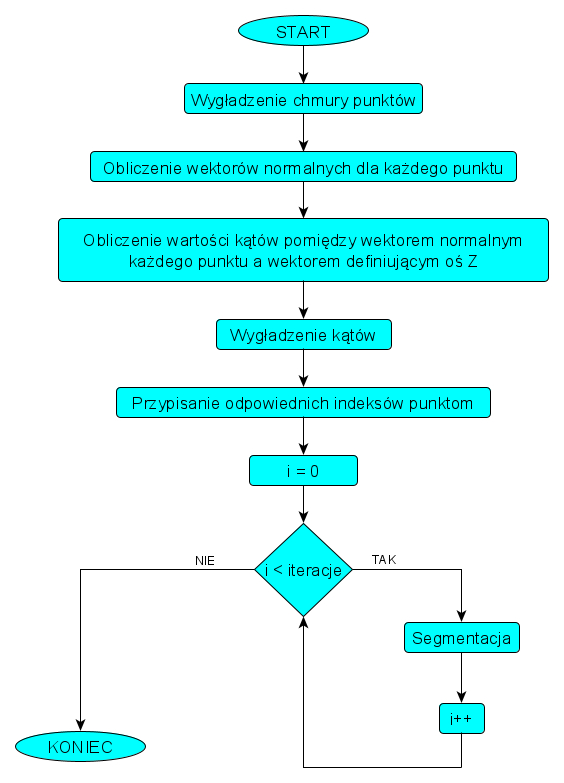
\includegraphics[width=0.85\textwidth]{algorythm.png}
		\caption{Algorytm działania programu}
		\label{fig:algorythm}
	\end{figure}
	
	Algorytm segmentacji działa w oparciu o odległości Hausdorfa. Odległością jest tu promień sąsiedztwa, który definiuje, ile punktów wraz z ich indeksami ma być wziętych pod uwagę podczas ustalania indeksu pojedyńczego punktu. Nie jest to jednak wierne odwzorowanie algorytmu odległości Hausdorfa\cite{pomerleau:hal-01178661}.\\
	
	\begin{figure}[h!]
		\centering
		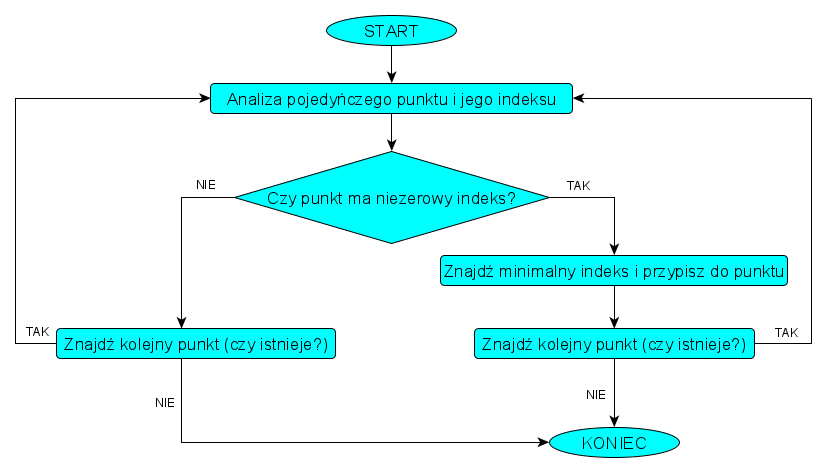
\includegraphics[width=\textwidth]{algorythm_of_segmentation.png}
		\caption{Algorytm segmentacji}
		\label{fig:algorythm_of_segmentation}
	\end{figure}